\section{Descrizione del progetto}
Per quanto riguarda la parte di \textit{ASM} si è deciso di riprendere un esempio visto in classe (e durante le pause caffè, molto amate da noi studenti), ovvero quello relativo alla \textit{\textbf{Coffee machine}}, che affiancherà il distributore di bevande energetiche progettato in Scala.

In particolare l'applicazione è stata definita basandosi su una serie di specifiche, quali:
\begin{itemize}
	\item Il distributore modellato può preparare \textbf{diverse tipologie di bevande} (caffè, cappuccino etc), ognuna delle quali è preparata con diverse quantità di ingredienti (acqua, caffè, latte etc) i quali vengono consumati dagli utenti e reintegrati dal manutentore;
	\item Il distributore accetta \textbf{pagamenti solamente in moneta} tramite l'inserimento di denaro nell'apposita fessura;
	\item Il distributore è in grado di fornire il resto;
	\item Quando tutte le bevande sono esaurite, il distributore va fuori servizio, in attesa che gli ingredienti vengano aggiunti dal manutentore, il quale può inoltre prelevare o inserire monete dal distributore, sempre tenendo conto del vincolo della capacità massima del vano porta monete
\end{itemize}
	

\section{Macchina a stati}
La ASM è basata su una macchina a stati finiti, mostrata in figura ~\ref{fig:StateMachine}, che definisce i principali stati e le principali transizioni che si possono verificare durante il funzionamento del distributore. 
\begin{figure}[h!]
	\centering
	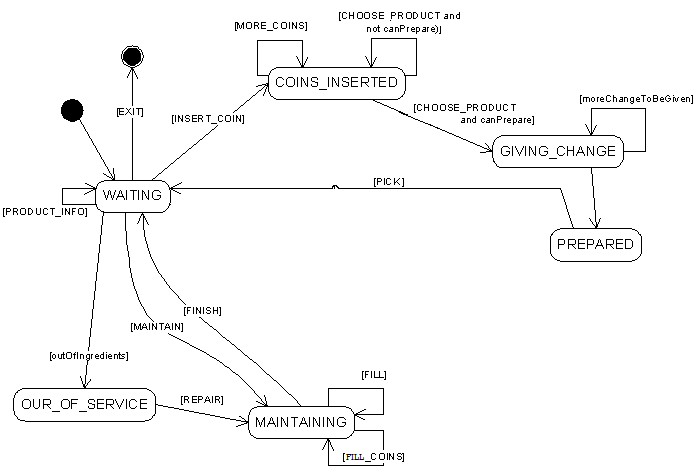
\includegraphics[width=0.6\textwidth]{Immagini/FSM.png}
	\caption{Macchina a stati}
	\label{fig:StateMachine}
\end{figure}

\newpage
\section{Eventi}
La ASM sviluppata modella un sistema event-driven, ovvero un sistema in cui le transizioni da uno stato all’altro sono perlopiù scatenate da input dell’utente, mentre di solito la macchina si trova ferma in uno stato, in attesa di tali eventi.

Nel codice ASMETA questi eventi sono denominati \textbf{action}: ad ogni stato corrispondono una o più azioni che l’utente può compiere quando la macchina si trova in quello stato, le quali sono codificate come elementi di un dominio enumerativo (figura ~\ref{fig:actionASM}).

\begin{figure}[h]
	\centering
	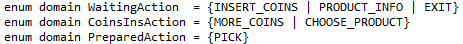
\includegraphics[width=0.6\textwidth]{Immagini/ActionASM.png}
	\caption{Action che implicano un possibile cambio di stato, qualora la condizione sia verificata}
	\label{fig:actionASM}
\end{figure}

La caratteristica event-driven del sistema si è riflessa nella ASM, infatti le regole (\textit{rules}) implementate possono essere suddivise in due categorie:
\begin{itemize}
	\item  regole che attendono il verificarsi di un’azione (qui chiamate \textbf{event management rules});
	\item regole di transizione (\textbf{transition rules}) che verificano la condizione della transizione e, se verificata, eseguono gli update opportuni per effettuare il passaggio di stato.
\end{itemize}
	
\textbf{In linea di massima, ad ogni stato corrisponde una \textit{event management rule}, mentre ad ogni arco (transizione) corrisponde una \textit{transition rule}.}

\section{Domini}
I domini introdotti nel codice ASM sono:
\begin{itemize}
	\item \textbf{Domini enumerativi}: per gli stati della FSM, uno per ciascun insieme di eventi (ciascun insieme contiene gli eventi validi per uno stato), ovvero quelli relativi alle possibili azioni eseguibili in ogni specifico stato, ed uno relativo alla tipologia di ingredienti utilizzati (figura ~\ref{fig:enumDomain});
	\item \textbf{Dominio statico concreto} per i tagli di monete riconosciuti dal distributore (in centesimi);
	\item \textbf{Dominio astratto} per i prodotti disponibili.
\end{itemize}

\begin{figure}[h]
	\centering
	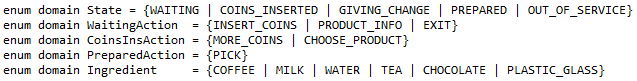
\includegraphics[width=0.5\textwidth]{Immagini/EnumDomain.png}
	\caption{Domini enumerativi}
	\label{fig:enumDomain}
\end{figure}

\section{Controlled - static - monitored functions}
\subsection{Controlled}
Le funzioni in figura ~\ref{fig:notMonitored}, rappresentano funzioni non-monitored così definite:
\begin{figure}[h]
	\centering
	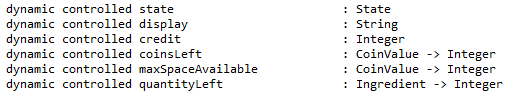
\includegraphics[width=0.5\textwidth]{Immagini/DynamicController.png}
	\caption{Funzioni non monitored}
	\label{fig:notMonitored}
\end{figure}

Si vede come le prime tre funzioni rappresentino delle funzioni 0-arie, ovvero delle variabili.

Le ultime tre funzioni invece sono n-arie, ovvero mappano dei valori da un dominio ad un codominio: nello specifico associano
\begin{itemize}
	\item coinsLeft: ad ogni Coins il numero effettivo di monete presente all'interno del distirbutore
	\item maxSpaceAvailable: ad ogni Coins associa il numero massimo di monete che il distributore può contenere
	\item quantityLeft: ad ogni Ingrediente un valore Integer, che non è altro che la quantità rimasta
\end{itemize}

I valori assunti dalle funzioni controlled rappresentano parte dello stato esteso delle ASM, quindi possono essere utilizzate per mantenere informazioni tra uno stato e l’altro della FSM.

\subsection{Static}
Le funzioni static (figura ~\ref{fig:staticFunc}) sono funzioni la cui interpretazione viene fissata dalla definizione della ASM e non può essere modificata durante l’esecuzione.
Possono essere paragonate alle costanti dei linguaggi di programmazione.
\begin{figure}[h]
	\centering
	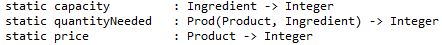
\includegraphics[width=0.5\textwidth]{Immagini/StaticFunction.png}
	\caption{Static functions}
	\label{fig:staticFunc}
\end{figure}
Per esempio la funzione \textit{price} rappresenta un legame costante tra un prodotto e il suo prezzo. 

\subsection{Monitored}
Le funzioni monitored rappresentano degli input che l’utente fornisce alla macchina. Il valore di queste funzioni non è persistente, ma viene ad essere specificato dall’utente per ogni stato tramite tastiera (oppure lette anche da file esterno, come fatto per i test automatici tramite file).
\begin{figure}[h]
	\centering
	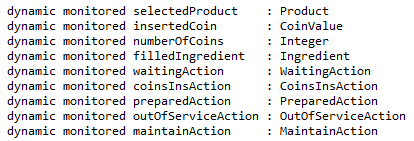
\includegraphics[width=0.8\textwidth]{Immagini/MonitoredFunc.png}
	\caption{Monitored functions}
	\label{fig:monitoredFunc}
\end{figure}
Tra le funzioni monitored figurano le funzioni che richiedono all’utente la scelta tra le azioni disponibili. Inoltre ci sono funzioni con cui l’utente specifica quale moneta, quale prodotto è stato selezionato e, per il manutentore, quale ingrediente è stato rifornito e quante monete ha lasciato nel distributore.

\section{Inizializzazione}
Di default, tutte le funzioni prendono valore undef per quei valori del dominio per cui non sono state esplicitamente definite.	
Perché la macchina inizi a operare in uno stato diverso, più significativo (anche perché raramente la macchina viene definita in modo da poter gestire valori undef), si deve inizializzare la macchina, ovvero definire uno stato iniziale, come fatto in figura ~\ref{fig:initialState}

\begin{figure}[h]
	\centering
	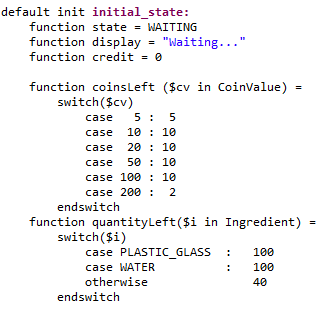
\includegraphics[width=0.5\textwidth]{Immagini/InitialState.png}
	\caption{Inizializzazione}
	\label{fig:initialState}
\end{figure}
In questo caso, lo stato FSM iniziale è quello di attesa, il credito in monete è nullo e la macchina possiede un discreto quantitativo di monete e ingredienti, per poter operare per un certo periodo senza bisogno di manutenzione.

\section{Event management rules e main rule}
Le event management rules si occupano di ricevere le azioni dell’utente e di eseguire (fire) la regola di transizione opportuna. In figura ~\ref{fig:managementRules} c’è un elenco delle regole, la cui struttura è del tutto simile a quella dell’unica regola definita. 

\begin{figure}[h]
	\centering
	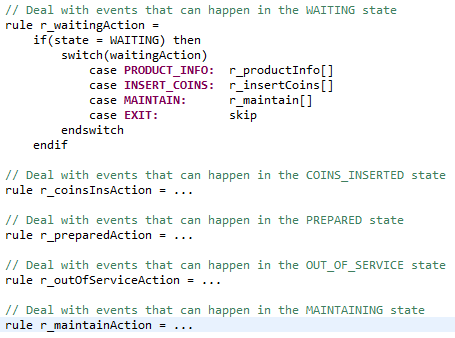
\includegraphics[width=0.5\textwidth]{Immagini/ManagementRule.png}
	\caption{Management rules}
	\label{fig:managementRules}
\end{figure}

La \textit{main rule}, che costituisce l’entry point del programma, controlla per prima cosa che il distributore possa operare, perché non ha finito gli ingredienti (r-selfCheck); questo è possibile grazie al comportamento del blocco sequenziale, che effettua gli update dopo la valutazione di ciascun termine. 

Dopo il controllo, invece, vengono valutate in parallelo le regole di gestione degli eventi: per esse non vi è pericolo di \textit{update inconsistenti} perché ciascuna regola ha una guardia che permette di valutare la regola solo quando la macchina si trova nello stato corretto (ogni regola si applica a un diverso stato, quindi sola una alla volta è “attiva”).

\section{Transition rule}
Ad ogni transizione della FSM, anche se rientrante sullo stesso stato, è associata una regola di transizione, che si occupa di valutare la guardia della transizione e, se questa risulta vera, di eseguire gli update opportuni, andando sostanzialmente ad effettuare un update dello stato.


\section{Simulazione}
La macchina è stata simulata con AsmetaS, sia in modalità interattiva che in modalità batch.
In modalità interattiva è facile scoprire errori sia di transizione di stato FSM sia di update, perché ad ogni update viene mostrato lo stato completo. Tuttavia una simulazione esaustiva è piuttosto lunga, per cui è difficile trovare errori nelle parti di macchina eseguite più raramente.

La modalità random permette di trovare facilmente violazioni inconsistenti: eseguendo una simulazione random con un numero elevato di transizioni (es. 1000) è più probabile coprire anche situazioni poco frequenti o poco naturali per un utente umano.

Per la simulazione batch è stato creato un file di environment testCoffee.env che esegue un tour più o meno completo degli stati e delle transizioni (della FSM).

Per facilitare questo tipo di simulazione è stato introdotta anche l’azione EXIT nel dominio WaitingAction, che è l’unica azione che produce un update set vuoto; è quindi possibile eseguire la simulazione batch con opzione –ne:

\textit{java -jar AsmetaS.jar -ne -env testCoffee.env CoffeeVendingMachine.asm}

